\chapter{Introduction}\label{ch:intro}

\section{The Nuclear Fuel Cycle}

The nuclear fuel cycle can be described as a set of facilities that interact
with one another to either provide or consume fuel services. Facilities in the
fuel cycle act together to provide fuel to nuclear power plants which, in turn,
generate energy. The used fuel produced by the power plants is then returned to
servicing facilities to either be recycled or disposed. The overall goal of the
system is to produce power at a competitive price while managing externalities
of the process, the chief of which is spent nuclear fuel. Myriad strategies
exist to achieve this aim which can be classified along a spectrum of the degree
to which fuel is recycled. In general, fuel cycles that do not recycle fuel are
concerned most with cost, whereas fuel cycles that fully recycle fuel are
concerned most with issues of sustainability and intergenerational equity. It is
the goal of fuel cycle simulation to rigorously explore this option space.

\subsection{The Open Fuel Cycle}
The open, or once-through, fuel cycle is relatively simple and is in place in
most countries in the world that currently utilize nuclear power. In practice,
the primary fuel element used in this type of cycle is uranium; however,
processed fertile material, such as thorium, can also be used. The fuel cycle is
considered open because fuel that is used in a reactor is stored indefinitely
once its reactivity has dropped below useful levels.

Beginning the fuel cycle process, uranium ore is initially extracted from the
ground using one of a variety of techniques including open pit mining,
underground mining, and \textit{in situ} leaching. The uranium ore is then
milled to form yellowcake, $\mathrm{U_3O_8}$. The tailings, or byproducts, of
this process are slightly radioactive and are therefore considered to be
low-level waste (LLW) by the Nuclear Regulatory Commission (NRC)
(see \cite{nrc_10_1985}).

Certain reactors are designed to use naturally enriched uranium. For these
reactors, yellowcake can be directly reduced with oxygen to form naturally
enriched uranium oxide, $\mathrm{UO_2}$. For the majority of power reactors,
however, the uranium must be enriched with higher-than-natural levels of
uranium-235. In order to do so, yellowcake is sent to a conversion facility,
which converts it from $\mathrm{U_3O_8}$ to $\mathrm{UF_6}$. The uranium
hexafluoride is then enriched to the required level in an enrichment facility,
of which three classes exist: gaseous diffusion, the original enrichment
technology; centrifugal diffusion, the current enrichment technology; and Atomic
Vapor Laser Isotope Separation (AVLIS), a newer technology not currently in
commercial production. The enriched uranium hexafluoride is then sent to a fuel
fabrication facility where it is returned to yellowcake form before being
reduced to uranium oxide. The uranium oxide is then sintered into pellets and
loaded into fuel assemblies to be placed in a reactor. This process, in
conjunction with uranium mining, is termed the \textit{front end} of the nuclear
fuel cycle.

Once fuel has been processed in a reactor, it is cooled off in pools for a
number of years, and then stored in dry casks before eventually being sent to a
final repository. The physical location of the fuel may vary during dry cask
storage between the reactor site or some other interim storage site.

Graphically, the open fuel cycle is shown in Figure \ref{fig:open-cycle}.

\begin{figure}[]
  \begin{center}
    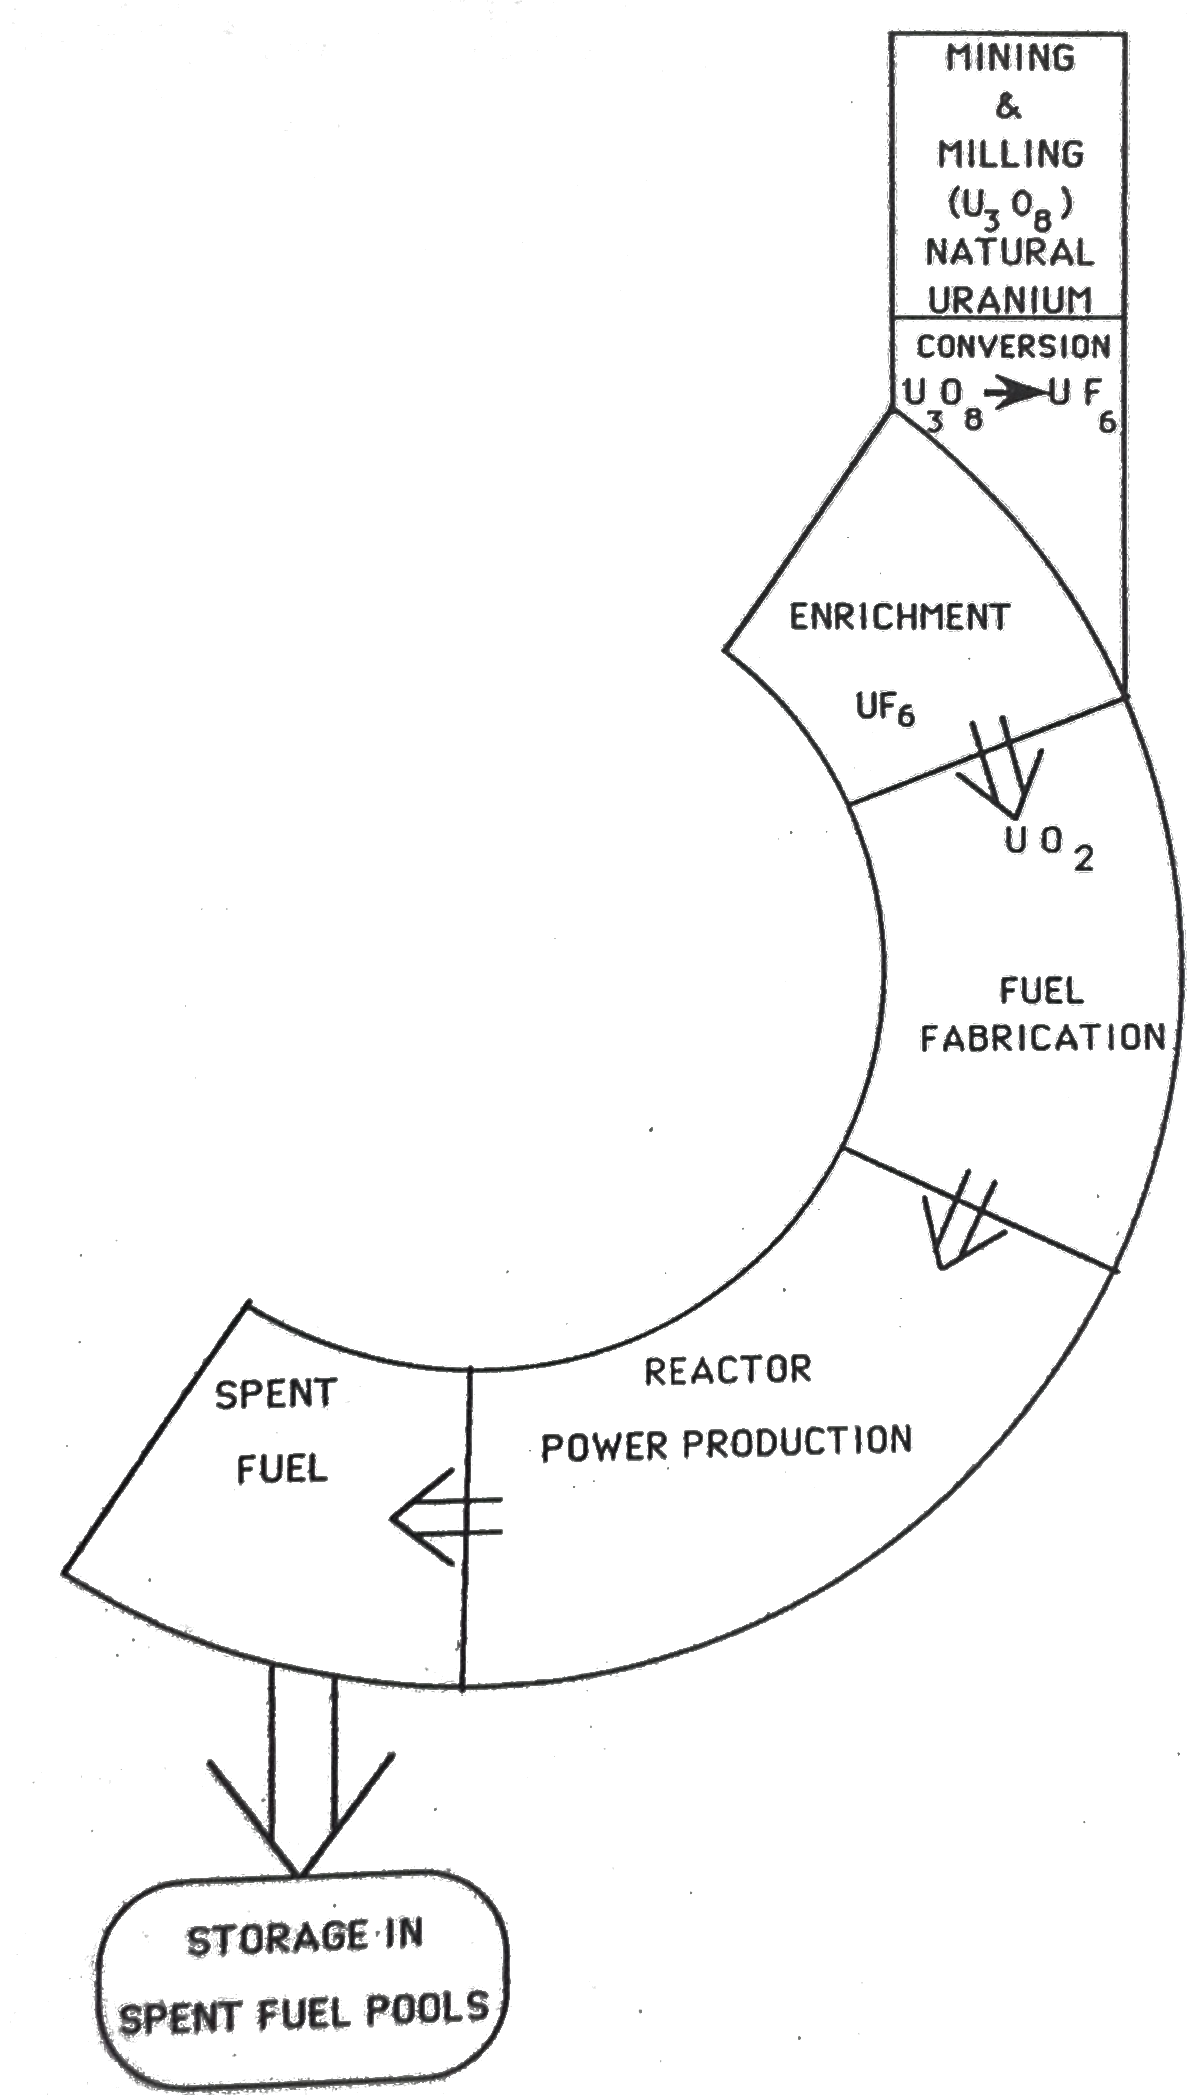
\includegraphics[height=7.5cm]{./chapters/intro/open_cycle.png}
  \caption{The once-through fuel cycle as shown in \cite{cochran1990nuclear}.}
  \label{fig:open-cycle}
  \end{center}
\end{figure}


\subsection{The Closed Fuel Cycle}
The closed fuel cycle is one that includes the recycling of used, or spent, fuel
to be reused in a reactor. Recycling used nuclear fuel is expensive due to the
costs associated with handling highly radioactive material (e.g., capital costs
of hot cells, etc.). However, there are at least two overarching benefits that
contribute to lowering the overall cost of the fuel cycle: increasing repository
capacity and increasing fuel utilization.

Spent fuel that exists the average Light Water Reactor (LWR) has an average
elemental makeup shown in Table \ref{tab:lwr_fuel}. Of the elements that
comprise used fuel, uranium, plutonium, and the mixed actinides (MA) are all
capable of producing power through the fission process. The fission products,
however, contain isotopes with high neutron capture cross sections, which
therefore act as poisons to the nuclear chain reaction. Achieving theoretical
100\% fuel utilization would thus require storing indefinitely only the fission
products and any other byproducts of the fuel cycle. Furthermore, repository
capacity is determined not only by total mass or volume, but also by heat load
and radiotoxicity, making the concentration of high-activity isotopes one of the
limiting factors in a repository's capacity. Fission products are generally
short-lived (in comparison to transuranic elements, i.e., uranium, plutonium,
and the MAs). Accordingly, by minimizing the amount of transuranics in a
repository, its capacity can be extended.

\begin{table} [h]
\centering
\begin{tabular} {|c|c|} 
\hline
Element Group & wt \% \\
\hline
Uranium           & $\sim$95  \\
Plutonium         & $\sim$1   \\
Mixed Actinides   & $\sim$0.1 \\
Fission Products  & $\sim$4   \\
\hline
\end{tabular}
\caption{Elemental Breakdown of Spent Fuel Exiting a Typical LWR}
\label{tab:lwr_fuel}
\end{table}

The act of reprocessing spent fuel is comprised of a number of
subprocesses. Once fuel has left the reactor core, it is stored in a spent fuel
pool for a some number of years, typically around five, in order to provide
enough time to lower decay heat to acceptable levels for handling of the
fuel. It can then be directly sent to a reprocessing facility or be sent for
some period of time to dry-cask storage. Reprocessing nuclear fuel is a chemical
extraction process and therefore is limited by chemical extraction
techniques. In general, there are two types of such processes: low-temperature
methods using organic solvents (e.g., PUREX), and high-temperature methods using
molten salts and metals, called pyroprocessing. The extraction techniques
separate the spent fuel into chemically-similar groups which can vary based on
the technique used, but generally align with those shown in Table
\ref{tab:lwr_fuel}. The separated streams are then sent either to a repository
as high-level waste (HLW) or to an appropriate fuel fabrication
facility. Graphically, the closed fuel cycle is shown in Figure
\ref{fig:closed-cycle}.

\begin{figure}[]
  \begin{center}
    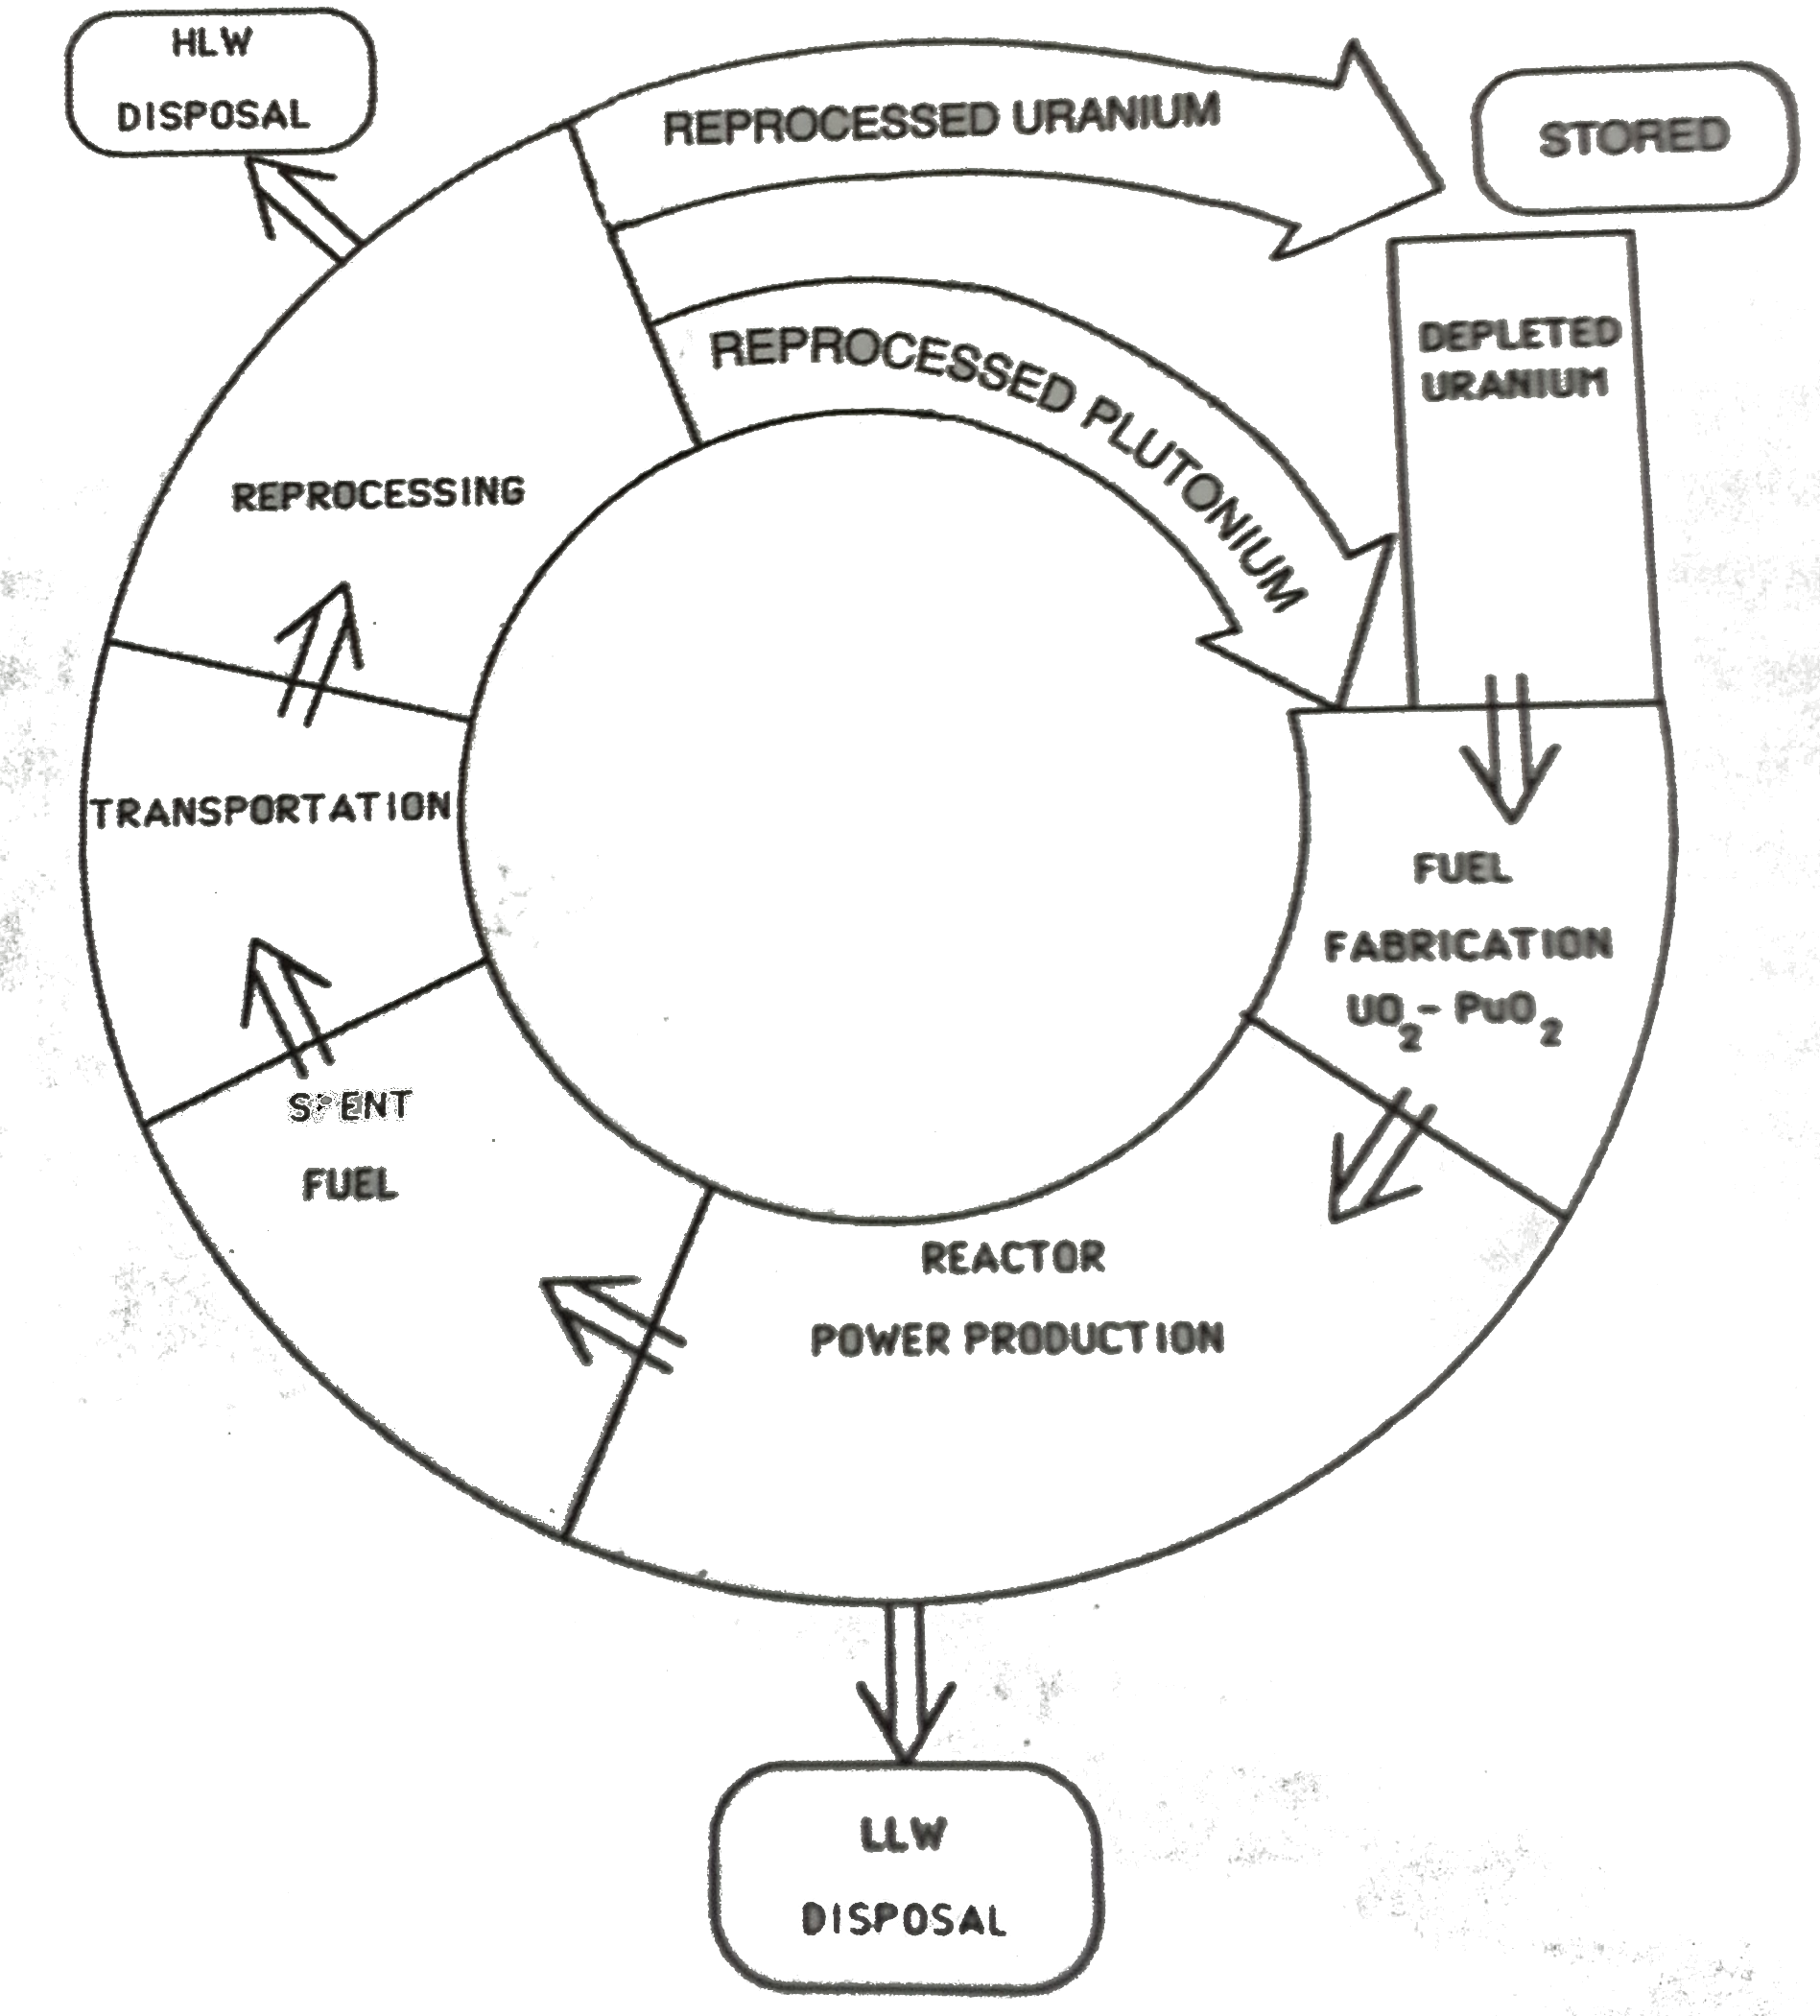
\includegraphics[height=7.5cm]{./chapters/intro/closed_cycle.png}
  \caption{The closed fuel cycle as shown in \cite{cochran1990nuclear}.}
  \label{fig:closed-cycl}e
  \end{center}
\end{figure}


The elemental groups used in fuel fabrication will depend on the fuel cycle that
is developed. The currently-operating large-scale industrial reprocessing plants
(La Hague in France, THORP in the U.K., Mayak in Russia, and Rokkasho in Japan)
utilize the PUREX process to extract uranium and plutonium. The plutonium is
then oxidized and mixed with depleted uranium from the enrichment process to
produce mixed-oxide fuel (MOX). Other sources of uranium can be used to fill MOX
fuel, such as recycled uranium from reprocessing, as neutronics-related
reactivity and safety constraints allow. Other fuel cycles utilize the mixed
actinides elemental group as well. Generally, plutonium is included with the
mixed actinides, which results in a elemental category called the transuranic
(TRU) elements. These fuel cycles generally include fast reactors that convert
their TRU inventory into either more TRU (i.e., they have a conversion ratio
(CR) of greater than 1), less TRU (CR < 1), or they maintain the amount of TRU
entering and exiting their system (CR = 1). Fast reactors with CR > 1 are termed
breeder reactors.

It should be noted that with any reprocessing capability, nonproliferation
issues arise. Nuclear weapons have historically been produced using either
enriched uranium or reprocessed plutonium; however it is possible to produce one
with any mix of appropriate materials. Accordingly, any fuel cycle that exposes
bare plutonium streams has an inherently higher nonproliferation risk than one
that does not, and such risks must be weighed accordingly. On a technical note,
though, the relatively low content of Pu-239, especially with respect to the
concentration of heat-producing Pu-240, in spent LWR fuel makes diverting such
fuel for the purposes of nuclear weaponry a route with an incredibly low
probability of success.


\subsection{The Modified-Open Fuel Cycle}
The modified open fuel cycle is effectively a hybrid of the open and closed fuel
cycles. The Blue Ribbon Commission's Reactor and Fuel Cycle
Technology Subcommittee tackled a definition as follows:

\begin{quotation}
We have defined this category to encompass a very wide range of possible fuel
cycles with multiple possible combinations of different reactor, separations,
and fuel fabrication technologies. Our definition includes any fuel cycle in
which some of the spent fuel is processed rather than being directly disposed of
after a single pass through a reactor.~\cite{brc_reactor_2012}
\end{quotation}

They mention, however, that there is no industry-wide agreed-upon
definition. For the purposes of this work I will use the committee's
definition. It should be noted that by the committee's definition, the French
nuclear power program is technically a modified-open cycle because MOX fuel
reprocessing has been demonstrated, but is not used at an industrial scale.


\section{Fuel Cycle Simulation}

\subsection{Overview}\label{sec:simulators-overview}
Fuel cycle simulation is a field with a variety of actors. The majority are
state-base (i.e., part of a government's national R\&D infrastructure), but
other players include universities as well as international governance
organizations such as the International Atomic Energy Agency (IAEA). The
modeling strategies applied to the nuclear fuel cycle span a wide range of
fidelity, both at the facility level and the material level. For instance, some
simulators describe reactors by fleet (or types) and solve material balances for
the entire fleet in aggregate while others instantiate individual (or discrete)
facilities. Similarly, some simulators make detailed calculations of fuel
depletion due to reactor fluence whereas others simply use pre-tabulated values
that depend (generally) on burnup values for thermal reactors and conversion
ratios for fast reactors.

There are, broadly, three decision categories that are of concern to fuel cycle
simulation. The first is facility deployment, specifically, how and why certain
facilities are deployed. There is general consensus regarding reactor deployment
in the community: a user defines an energy growth curve and, for each type of
reactor in the simulation, a percentage of that total energy demand to be met by
the reactor type. However, the nuclear fuel cycle is a special case of
supply-demand modeling where certain facilities (e.g., fast reactors) require
fuel that has been processed by other facilities (e.g., thermal
reactors). Accordingly, simulation developers must make a choice: should one
allow a facility to be built if it may not be able to be fueled? Certain
simulators explicitly disallow this behavior by determining reactor build
decisions based on lookahead algorithms (e.g., CAFCA, VISION), others explicitly
allow it (e.g., COSI), while still others offer a hybrid approach that allow a
lookahead function based on a certain amount of fuel that will eventually be
needed over a reactors lifetime (e.g., DANESS). The eventual choice of this
decision making process greatly affects simulation outcomes in any scenario in
which a lack of fuel exists. Because these simulation tools are built to analyze
the dynamic symbiotic relationship between different reactors in a cyclical
process (e.g., thermal and fast reactors), among other scenarios, this
simulation development decision is arguably very important to simulation
outcomes.

The second major simulation development decision is determining fuel
isotopics. A number of complications are encompassed in this decision. As an
example, consider MOX fuel for thermal reactors. In general, MOX fuel is
composed of oxide forms of plutonium (and some minor actinides, such as
americium) from spent thermal fuel as well as uranium (the source of which can
be depleted enrichment tails, depleted recycled uranium or natural uranium). The
fact that depleted uranium, rather than enriched uranium, can be used stems from
the fact that the separated plutonium is largely comprised of fissile isotopes
(\nucl{239}{Pu} and \nucl{241}{Pu}). The source of uranium already introduces an
isotopic dependency of importance: the \nucl{235}{U} enrichment of the fill
uranium should affect either the quantity of plutonium used, the isotopics of
plutonium used (with higher \nucl{235}{U} enrichment implying a lower
concentration of fissile plutonium isotopes), or both. Further complicating the
issue is that plutonium isotopes are radioactive and decay on (relatively) short
time scales. For instance, the half life of \nucl{241}{Pu} is $\sim$14
years. Accordingly, the quality, or isotopic content, of the separated plutonium
changes on a time scale on the order of the simulation due to decay. There is a
similar issue with other transuranic radioactive isotopes of interest to nuclear
fuel cycles.

Accordingly, simulation developers have two general choices with respect to
input fuel isotopics (and isotopic-level modeling in general). The first is
whether or not to include isotope decay. As might be expected, the simulators
fall into two camps, those that include decay (e.g., VISION and COSI) and those
that do not (e.g., DANESS and CAFCA). Interestingly, the MIT development team
claims that the lack of modeling decay does not affect the simulation as long as
all transuranic isotopes are lumped together \cite{guerin_impact_2009}. Other
codes appear to include isotopic decay in order to inform output metrics such as
repository heat capacity. The second choice involves matching input isotopics
with available separated isotopes. This is an interesting problem because
separations technology work on a elemental scale, whereas input fuel recipes are
defined on an isotopic scale because neutronics properties are functions of
individual isotopes rather than elemental aggregates. In other words, you can't
change the separated plutonium isotopic vector to match a recipe, as one does
with uranium enrichment (which is an isotopic-scale process). A full treatment
of the problem is relatively complicated and requires mixing separated plutonium
vectors to find a ``best match''; this problem has been termed the Winery
Problem or the Recipe Approximation Problem \cite{oliver_geniusv2:_2009}. The
current generation of fuel cycle simulators generally punt on this issue. A
common strategy is to declare a target subset of isotopics, normally a specific
plutonium isotope or the aggregate plutonium isotopes, and match quantities of
that set. For example, if the set is of single cardinality (e.g.,
\nucl{239}{Pu}), then the amount of that isotope is guaranteed to be correct,
but accompanying isotopics are not. On the other hand, if the set is a group of
isotopes (e.g., all plutonium isotopes), that group's quantity is guaranteed to
be correct, but the specific isotopics are not. One can conclude from this
discussion that the level of isotopic detail modeling in a simulation could
greatly affect the outcome of the simulation, especially if decisions are made
mid-simulation regarding the isotopes in question (e.g., whether or not to build
a fast reactor given the available amount of separated isotopes). A full
treatment of how the current generation of simulators tackle this issue is
described in \S\ref{sec:simulators}. An overview of the proposed strategy to
take in the \Cyclus simulation environment is described in \S\ref{sec:rap}.

The third major development decision is how to determine connections between
facilities. At issue here is how servicing facilities (e.g., fuel fabrication
facilities) are connected to serviced facilities (e.g., reactors). For those
simulators that do not model discrete facilities (e.g., CAFCA), the modeling
technique is relatively trivial: a fleet of servicing facilities are directly
connected to their serviced facilities. If more than one type of facility is
being serviced (e.g., TRU-based fuels going to thermal and fast reactors), then
a user must define the percentage of capacity going towards each type of
serviced facility \cite{busquim_e_silva_system_2008}. A similar situation arises
in other systems-dynamics based simulators, because mass flow balance equations
govern the inner workings of the simulations. This situation becomes even more
complicated if regional scenarios are to be modeled. In addition to determining
which serviced facilities will be connected to servicing facilities, one must
also incorporate a notion of the region of serviced and servicing
facilities. DESAE includes a rather simplistic model of this relational nature
that predetermines the yearly intra-regional trading \cite{iaea_nuclear_2010}. A
full treatment of this class of developmental decision making with respect to
the current set of fuel cycle simulators is provided in
\S\ref{sec:simulators}. An overview of the proposed strategy to take in the
\Cyclus simulation environment is described in \S\ref{sec:rap}.


\subsection{Metrics}
Fuel cycle simulators have a number of possible output metrics of interest, and
the Department of Energy has initiated a number of exercises to discuss them
through its Used Fuel Disposition campaign \ref{nutt_proposed_2012,
taiwo_summary_2012}. One of the original reasons that fuel cycle simulators were
developed was to determine the relative cost of different fuel cycles. The
notion of fuel cycle cost can either be calculated in a post-processing step, or
it can be calculated on-the-fly during a simulation. The benefit of maintaining
cost information during a simulation is that the simulation can react to these
costs. A prime example of such behavior is in the DANESS simulation code,
described in \S\ref{sec:other-sims}. Other simulators, such as VISION, determine
costs at the end of a simulation based on all events in the simulation using
values from AFCI cost basis report
\cite{yacout_vision_2006,shropshire_advanced_2007}. It must be stressed that the
notion of predicting future fuel cycle costs have a high degree of
variability. They depend not only on the level of maturity of technologies as a
function of time (i.e., the R\&D investment level for the technology), but also
on material costs which are relatively unknown and/or very hard to
predict. Accordingly, it helps to determine relative costs of fuel cycles rather
than absolute costs of fuel cycles. Further, it helps to classify fuel cycles by
the technology used in them.

The fuel cycle cost metric provides a prime example of a key choice of
developers of fuel cycle simulators. Most metrics outside the actual
instantiation of facilities (i.e., which facilities are built when) and the flow
of material, which are integral to the running of the simulation, can be post
processed. They are only required to be maintained during the simulation if the
some aspect of the simulation depends upon them. Accordingly, unless decisions
are being made on the basis of costs, there is no reason to maintain a cost
metric at simulation time. Simulators can generally be divided into two groups,
those that make decisions at run time based on certain metrics and those that do
not. \Cyclus is designed to provide dynamic support of metric-based decision
making, e.g., Huff's recent work with dynamic repository capacity determination
\cite{huff_integrated_2013}.

A large number of metrics related to fuel cycle simulation come directly from
the material mass flows. For instance, proliferation based metrics are generally
determined by the amount of separated transuranic material at any point in the
fuel cycle. Metrics that lead to less proliferation resistance include the
amount of significant quantities of material, defined by the IAEA to be the
quantity of any given material (e.g., TRU or plutonium) sufficient to make a
nuclear weapon. These are generally defined on the elemental level, which
ignores realities based on isotopic dependencies (e.g., \nucl{240}{Pu} is a
relatively large source of decay heat and is thus reduces the aggregate
plutonium's effectiveness for use as a weapon). Metrics that lead to more
resistance of proliferation activities include the unshielded dose rate of a
given material, which makes handling (and thus diverting) the material more
difficult \cite{yacout_vision_2006}. Another key metric that is important to
many in the fuel cycle simulation community is uranium utilization. At present,
the United States political stance is to continue the once-through fuel cycle
until it is economically viable to begin reprocessing spent fuel for recycle in
reactors \cite{hamilton_blue_2012}. Such a situation can only arise if the
supply of uranium dwindles to a low-enough level which will raise the price of
uranium sufficiently to make reprocessing a viable alternative. It is
additionally interesting to note the approximate time at which uranium capture
from sea water, which is in developmental stages, will become economically
viable. These situations all depend on the amount of uranium used in a given
simulation, which is, of course, related to fuel mass flows.

Another key output of simulators is related to repository capacities. The
capacity a repository to store spent fuel could be reached in a number of
ways. Spent fuel isotopics, especially fission products, produce a large amount
of decay heat which can reach the thermal limits of their containers over short
periods of (geologic) time. There are also radiotoxicity limits for repositories
in order to limit the risk of radiological releases. Finally, there are mass and
volume limits on repositories, representing a space storage capacity. In fact,
the Nuclear Waste Policy Act, the current U.S. law determining the U.S.'s used
fuel management strategy, places a blanket mass capacity limit of 70,000 t on
Yucca Mountain \cite{us_nuclear_1982}.  It is not clear at the current time
which of these limiting capacities will ultimately be the governing
engineering-based limiting factor for repositories. Furthermore these capacities
change based on repository layout and geology.  This parameter was key in
Scopatz's work with static fuel cycle simulation
\cite{scopatz_essential_2011}. In all cases, these capacities can be calculated
in terms of isotopic quantities of waste products. It is possible to calculate
the capacity parameters \textit{in situ} during the simulation, shown by Huff in
\cite{huff_integrated_2013} and dynamically alter the simulation based on the
results rather than simply performing a post-processing operation to report the
required number of repositories for the simulation.


\section{Open Questions in Fuel Cycle Simulation}
\subsection{Using Agent-Based Models}

Stepping back a moment from the discussion of nuclear-specific fuel cycles, the
interactions that we wish to model are those of supply and demand. Certain
facilities need some sort or raw or processed material that other facilities
produce. The fuel cycle is more complicated than this simple statement, though,
because facilities are connected through recycled fuel. Even with such a
complication, the notion of a generic fuel cycle, i.e. from the perspective of
facilities that supply and demand material, quickly begins to look like a supply
chain model. There is a growing literature of agent-based supply chain modeling
\cite{swaminathan_modeling_1998,julka_agent-based_2002,van_der_zee_modeling_2005,chatfield_multi-formalism_2007,holmgren_agent_2007}.
The general premise of these types of models is that individual facilities have
a notion of their needs (i.e., their demands) and can express to the system
these needs at the required time. There is heavy use of inventory policy to
determine the correct amount of material inventory that is needed and the
correct time to request a resupply. In general, a facility may be comprised of
many agents, e.g. an ordering agent, a stocking agent, a forecasting agent,
etc. Such an approach has not heretofore been attempted for the nuclear fuel
cycle and opens up a variety of doors. For example, reactor facilities could be
allowed to be fueled by multiple fuel types (e.g., UOX or MOX), and decide which
type to choose based on the simulation environment. However, due to the
fungibility of material in the fuel cycle (plutonium, for instance, can be used
by fast reactors and thermal reactors), many questions remain about how to
describe the materials to be traded and the markets on which they will be
traded. A more fully formed proposal for such a treatment is presented in
\S\ref{sec:gfctp}.

\subsection{Input Fuel Isotopic Matching}

One of the major issues with current fuel cycle simulation is the disconnect
between fuel recipes being requested by reactors that need recycled fuel,
e.g. MOX fuel. The isotopics that comprise these materials, especially the
transuranic isotopes, are radioactive, and thus the actual isotopic composition
of material change with time. Accordingly, if a simulator wishes to try to match
the requested isotopics, it must keep track of the decay of isotopes. Further
complicating the problem is that requested input fuel recipes may not
necessarily be related to the provided output fuels, i.e., there is a mismatch
between the output isotopics and input isotopics even without the presence of
isotopic decay. The majority of fuel cycle simulators to date ignore this issue
and instead choose to match recipes ``exactly'' based on a subset of
isotopes. Further details of how other simulators tackle this issue are reviewed
in \S\ref{sec:simulators}. A full treatment of the recipe-matching problem would
require an approach similar to the pooling-blending problem
\cite{tawarmalani_convexification_2002}. There is a rich literature base for
pooling-blending problems
\cite{glen_mixed_1988,rigby_evolution_1995,mendez_simultaneous_2006,misener_advances_2009}
in the industrial processes literature. However, the majority of the subject
matter concentrates on refinery operations such as mixing various crude oils to
hit a certain octane level. These are (relatively) simple problems because the
properties that are trying to be matched are extrinsic and linear function of
the mixing variables. The nuclear arena is much more complicated because of
criticality limitations and the want to match aggregate nuclear properties of
materials. Accordingly, a hybrid approach was proposed that involves blending and
approximation theory. The approach is outlined in \S\ref{sec:rap}.

\subsection{Modeling Global Regions}

The notion of regional modeling in fuel cycle simulation has always been a
secondary concern. Certain simulators attempt to model it explicitly, e.g. DESAE
\cite{iaea_nuclear_2010}. Other simulators have attempted to add the capability
at some point after their simulator had already been developed, e.g. VISION and
COSI. A discussion of these capabilities follows in \S\ref{sec:simulators}. Some
semblance of this capability is needed if one is to incorporate outside effects
on a domestic fuel cycle. Furthermore, a robust capability is required if one
wishes to actually investigate dynamic interactions amongst regional
entities. Again, a full treatment of this sort of regional interaction would
require international relations models, most of which can be found in the
cross-cutting realm of economics, political science, and game theory. The
primary solution technique is called Nash Equilibrium, and effectively describes
an optimal solution as follows: given a set of players, states, preferences,
and actions, all players choose an action such that any single player's
deviation from that actions results in a state of lower preference for that
player (thus no player has an incentive to deviate)
\cite{mccarty_political_2007}. There also exists a body of literature that
examine Nash Equilibria in the context of optimal flow models
\cite{mazumdar_fairness_1991,nagurney_supply_2002,song_nash_2002}. However, the
complexity of such models quickly brings them out of the scope of our needs,
i.e., dynamic modeling of multi-lateral scenarios ranging 100+ years in a
short-time ($\sim$2-5 minutes). Accordingly, a market resolution mechanism has
been proposed that allows for interaction amongst the various facilities and
managing entities (e.g. their regions). In order to inform a cardinal preference
\cite{strotz_cardinal_1953} relation for a facility over its possible supply
materials. The full approach is outlined in sections \S\ref{sec:gfctp} and
\S\ref{sec:agent-interaction}.

